\chapter{Search for semi-visible jets}  % might want to be more specific with the title if it only considers the generator-level studies
\label{chap:svj}

\epigraph{Of darkness visible so much be lent, as half to show, half veil, the deep intent.}{--- Alexander Pope}

\initial{T}his is the analysis chapter on \glspl{svj}.  % Obviously, write a better introduction to the chapter

%=======
\begin{easylist}[itemize]
    \easylistprops
    & Not 100\% sure whether this should go between theory and detector chapters, between detector and objects, or between objects and Hinv.
    && This could even be appended onto to the SVJ bit in the theory chapter, instead. Though, there would be a reasonable amount of material and discussion, so probably deserves its own (short) chapter
    & Only really discuss my contributions: $s$- and \tchannel signal model production and understanding. Can go into reasonable detail -- at the level of the AN or perhaps deeper
    && Show a few distributions from \tchannel signal, just for some insight as to how they differ from \schannel. Not sure if they need some sort of approval since they're generated with \acrshort{cmssw}
    && Objects (AK4 jets, AK8 jets, MET) are straight out of nanoAOD, without the further processing and quality cuts that go into the Hinv objects. Though, since the objects have gone through the full CMSSW processing pipeline, there should be at least some intrinsic level of quality of the objects.
    && Also say that my \MADGRAPH implementation has been built upon for the upcoming \tchannel and boosted \PZprime searches
    & Perhaps give a brief summary of the analysis: dijet search, using an SVJ tagger, transverse mass as fit variable. Say that details/complete description is discussed in the paper/Giorgia's thesis (with references)
\end{easylist}

% Can pull from Section 35 of my lab book, and all the talks I and other people from the team have given (Presentations and talks/ folder, also Other peoples/ subdirectory). Can also pull from AN for theory, translation of some theory stuff into experiment, and analysis strategy

% Could send a copy of the thesis to the SVJ team once I've got a complete first draft of this chapter. They would only need to look at theory section for SVJ, and this chapter. But I'd probably want to send the whole document since there are references to sections/formulae elsewhere in the thesis, and links would break, otherwise


%=========================================================


\section{Analysis summary}
\label{sec:svj_overview}

% Can just say it's a dijet search, using MT as search variable (better resolution than dijet mass). Can just reference Giorgia's thesis and say the rest of the info is there. Then can end section by saying my work was primarily on signal simulation. Developing MadGraph implementation to verify and cross check against Pythia implementation in s-channel, and be able to produce t-channel samples in preparation for a t-channel analysis. Code is being used for t-channel search now (still in preliminary stages), and also for a low mass boosted Z' search


%=========================================================


\section{Signal simulation}
\label{sec:signal_sim}

In the main analysis for the \schannel signal model, \PYTHIA is used as it can parametrise all the relevant aspects of the model in a simple manner with high signal efficiency. \MADGRAPH is the often-preferred generator as it can handle more complex models and decays. A higher degree of customisation and tuning of parameters is also possible. For the \schannel mode, the scattering matrix element calculations that model the hard process are identical between \PYTHIA and \MADGRAPH. In the former, the characterisation, interactions, and decays of the dark sector particles are implemented via the \texttt{Hidden Valley} module, available from \PYTHIA~8.226. Samples generated with \MADGRAPH are hadronised by \PYTHIA as part of the full simulation chain within \acrshort{cmssw}. \Gls{jet} matching and filter efficiencies may noticeably reduce the final number of events. The \tchannel model is possible to parametrise in \PYTHIA, but due to its complexity, we opt to do so in \MADGRAPH. Hadronisation, however, is still performed by \PYTHIA. In all cases, signal samples are generated at \acrfull{lo}.

% Not sure if Pythia actually does a matrix element computation, I basically just got the phrase from Kevin. Maybe I should change it to something like "the hard process should be equivalent between \PYTHIA and \MADGRAPH at LO", or smth.

The full description of \schannel signal generation with \PYTHIAEIGHT is given in Chpts.~\ref{subsec:svj_signal_pythia} and \ref{subsec:svj_showering_pythia}. An equivalent implementation where the hard scatter is modelled in \MGvATNLO, as both an alternative and cross-check to the \PYTHIA [version], is [described] in Chpt.~\ref{subsec:svj_signal_madgraph}. A description of the \tchannel process is also present. Comparisons between the \PYTHIA and \MADGRAPH implementations are [given] in Chpt.~\ref{subsec:svj_schannel_comparisons}.

% Mention these signals are generated privately? And that colleagues at Fermilab, Zurich, and Maryland designed the Pythia production while I handled MadGraph?

% Maybe make a note that most plots in this chapter are generated using 2016 conditions. The analysis began in 2017, and as such, when signal, background and data were being studied, the only complete dataset was 2016. And as that was the most mature dataset (been studied most by the Collaboration, so it was understood well), it was a good starting point. Selecting one year also ensures consistency, even though just showing signal MC shouldn't significantly change year-to-year
%  - What I could do, in principle, is just scale the 2016 plots to 137 fb-1 to avoid answering the above. Or, to be more correct, generate 2017 and 2018 samples for these mass points and scale them to their respective lumis, then combine them for a full Run-2 picture


%=========================================================


\subsection{Generation in \texorpdfstring{\MADGRAPH}{MadGraph}}
\label{subsec:svj_signal_madgraph}

The \MADGRAPHFULL event generator~\cite{Alwall:2011madgraph} is able to simulate the hard scatter for both the $s$- and \tchannel aspects of the \gls{svj} signal, i.e., the decay of the \PZprime into $\Pqdark\Paqdark$ in the \schannel mode, and the exchange of the $\PBifund$ to transform $\Pquark\APquark$ into $\Pqdark\Paqdark$ in the \tchannel mode. Up to two additional \acrlong{sm} quarks or gluons may accompany the final state for both modes. The particles, couplings, and other parameters required to describe the models are defined using the \FEYNRULES package~\cite{Alloul:2013bka}. Of the four principal free parameters the model in Chpt.~\ref{subsec:theory_svj_free_params}, the mediator mass and \mqdark are defined at this stage.

The \schannel process is a modified version of the spin-1 ``DMsimp'' class of simplified dark matter models~\cite{Backovic:2015soa}. The \tchannel description is completely custom. Both were initially acquired by the analysis team from one of the authors of Ref.~\citenum{Cohen:2017pzm}at \url{https://github.com/smsharma/SemivisibleJets}. At the time, it contained only one set of mass points. I have since greatly expanded on both models, allowing any combination of \PZprime, $\PBifund$, and \Pqdark masses and couplings. All signal samples produced with \MADGRAPH that feature in this thesis were done so with \url{https://github.com/eshwen/SemivisibleJets}. % Removing space between "Ref.~\citenum{Cohen:2017pzm}" and "at" otherwise it adds double space

In addition to the hard process, the full \acrshort{cmssw} simulation pipeline can also be executed. This allows for hadronisation and decays of both the \acrshort{sm} and dark quarks in \PYTHIA (as detailed in Chpt.~\ref{subsec:svj_showering_pythia}). The remaining free parameters of the model---\aDark and \rinv---are specified there. Subsequently, detector conditions and material interactions can be modelled in the 2016, 2017, and 2018 data taking periods of \acrshort{cms}. The parton distribution functions used in centrally-produced \acrshort{cms} simulation for each data taking period are also applied to these \gls{svj} samples for consistency.

Common to both the $s$- and \tchannel signal models generated for these studies, the couplings between the mediator and \acrshort{sm} quarks \gq---also the mediator and dark quarks \gqdark---are set to 1.0. Coupling strengths are furthermore independent of the dark and \acrshort{sm} quark flavours. The number of dark flavours \Nf and dark colours \Nc each have values of 2. Both affect the dark force scale as per Eq.~\ref{eq:lambda_dark}. Individually, former parameter allows for the production of two types of dark hadron, described in Chpt.~\ref{subsec:svj_showering_pythia}, while the latter sets the dark colour composition of the dark gluon \Pgdark. 


%=========================================================


\subsubsection{\texorpdfstring{\MADGRAPH}{MadGraph} run settings}
\label{subsubsec:svj_mg_run_settings}

Somewhat decoupled from the parameters of the signal models themselves, there are many important, adjustable settings controlled by the run card that affect the behaviour of \MADGRAPH. The most notable of which is the parton/\gls{jet} merging scale, denoted as the \texttt{xqcut}. \MADGRAPH has difficulty simulating soft, collinear physics. To avoid this, a threshold may be placed on the \texttt{xqcut} to only generate sufficiently energetic events. Between two partons $i$ and $j$, the \kt is given as
\begin{equation}
    \kt^2 = 2 \min(p_{\mathrm{Ti}}, \ p_{\mathrm{Tj}}) [\cosh(\eta_i - \eta_j) - \cos(\phi_i - \phi_j)]
    \label{eq:svj_mg_kt}
\end{equation}

where $\eta$ and $\phi$ are the pseudorapidity and azimuthal angle, respectively. Complete definitions are presented in Chpt.~\ref{subsubsec:geometry}. Events with $\kt < \texttt{xqcut}$ are not simulated. In essence, the \texttt{xqcut} is a measure of the required separation between partons in the event. We set a value of 100\GeV in the analysis for consistency with Ref.~\citenum{Cohen:2017pzm}. This interpretation of a merging scale is similar, but not quite the same, as \PYTHIA's discussed in Chpt.~\ref{subsec:svj_showering_pythia}.

The choice of the parton distribution function also lives in the run card. As stated above, this parameter changes based on the data taking period we emulate. Preferences for particle separation, momentum and direction cuts, beam energy, and the \acrshort{qcd} renormalisation and factorisation scales are some of the additional settings that can be customised.


%=========================================================


\subsubsection{\texorpdfstring{\schannel}{s-channel}}
\label{subsubsec:svj_signal_madgraph_schannel}

In the description of the \schannel model, the leptophobic \PZprime is a spin-1 boson with vector couplings to the dark and \acrshort{sm} quarks. A width $\Gamma_{\PZprime} = \text{10}\GeV$ is specified. The dark quarks themselves are Dirac spinors with dark colour quantum numbers. Real and complex scalar dark quarks also exist in the files [describing] the model, but are decoupled and not generated in our implementation. Consideration of these [additional] types of particle are beyond the scope of this thesis.

Cross sections for this process are calculated as a function of \mZprime, assuming resonant production and a universal quark coupling. Those given by \MADGRAPH are far too large and appear unrealistic. % Tracing back through the code used to calculate the cross sections, and what I think is the paper Nhan Tran was on for the dijet search, I think the cross section calculation comes from https://arxiv.org/abs/1306.2629, maybe more explicitly from slide 68 of https://indico.cern.ch/event/818454/contributions/3418046/attachments/1866479/3069375/CMS_PF_June20.pdf

It is important to understand the influence each free parameter of the model exerts on the kinematics of the final state particles. In which observables the variations of a given parameter manifest can aid in disentangling potential signal from background. The sensitivity, or lack thereof, of a parameter on the search variable also creates a sensible range for which to constrain the set of signal samples that must be generated. Signal models are given a label as SVJ\_\-$\expval{m_{\mathrm{mediator}}}$\_\-$\expval{\mDark}$\_\-$\expval{\rinv}$\_\-$\expval{\aDark}$. A benchmark point was chosen in the analysis with $\mZprime = \text{3000}\GeV$, $\mDark = \text{20}\GeV$, $\rinv = \text{0.3}$, and $\aDark = \text{peak}$, labelled as SVJ\_\-3000\_\-20\_\-0.3\_\-peak. Fig.~\ref{fig:svj_mg_benchmark_variations} shows the transverse mass of the dijet system \mT in the case where a single free parameter was varied with respect to the benchmark point. A glimpse into the sensitivity of the parameter on the kinematics is evident.

% Why do we use SVJ_3000_20_0.3_peak as a benchmark? Check the AN

\begin{figure}[htbp]
    \centering
    \begin{subfigure}[b]{0.48\textwidth}
        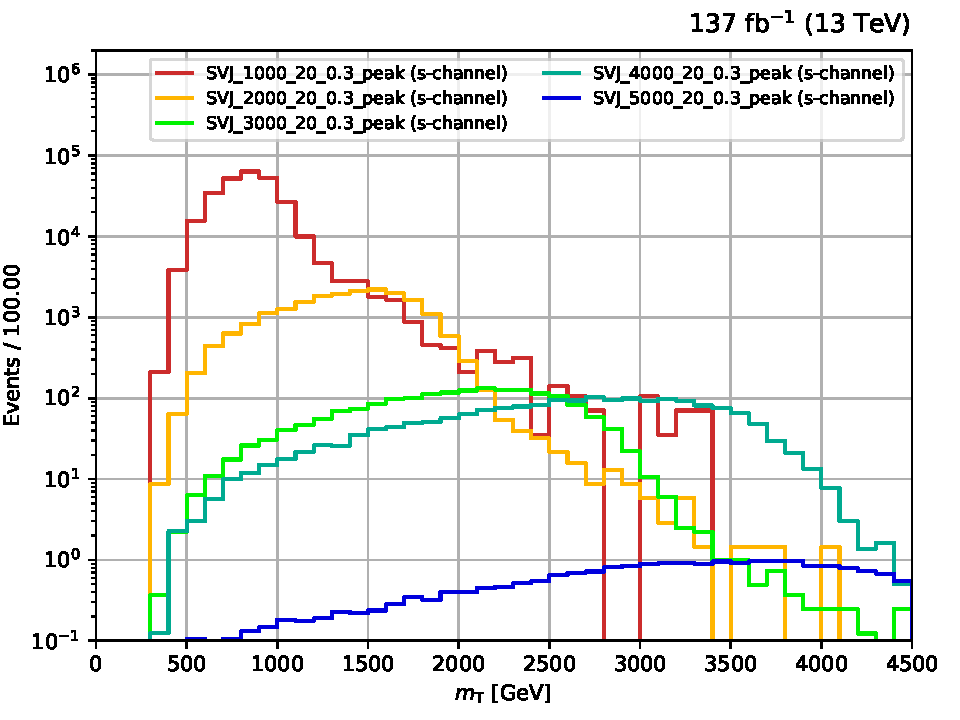
\includegraphics[width=\textwidth]{figures/s_channel_benchmark_variations/mZp.pdf}
        \caption{Varying \mZprime}
    \end{subfigure}
    \hfill
    \begin{subfigure}[b]{0.48\textwidth}
        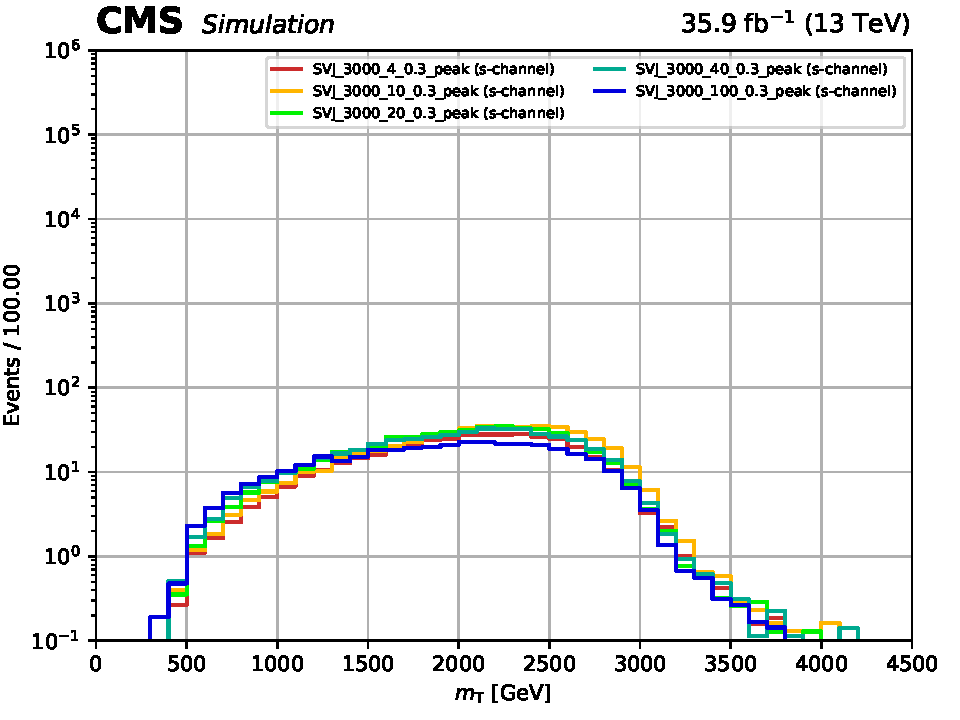
\includegraphics[width=\textwidth]{figures/s_channel_benchmark_variations/mD.pdf}
        \caption{Varying \mDark}
    \end{subfigure}

    \begin{subfigure}[b]{0.48\textwidth}
        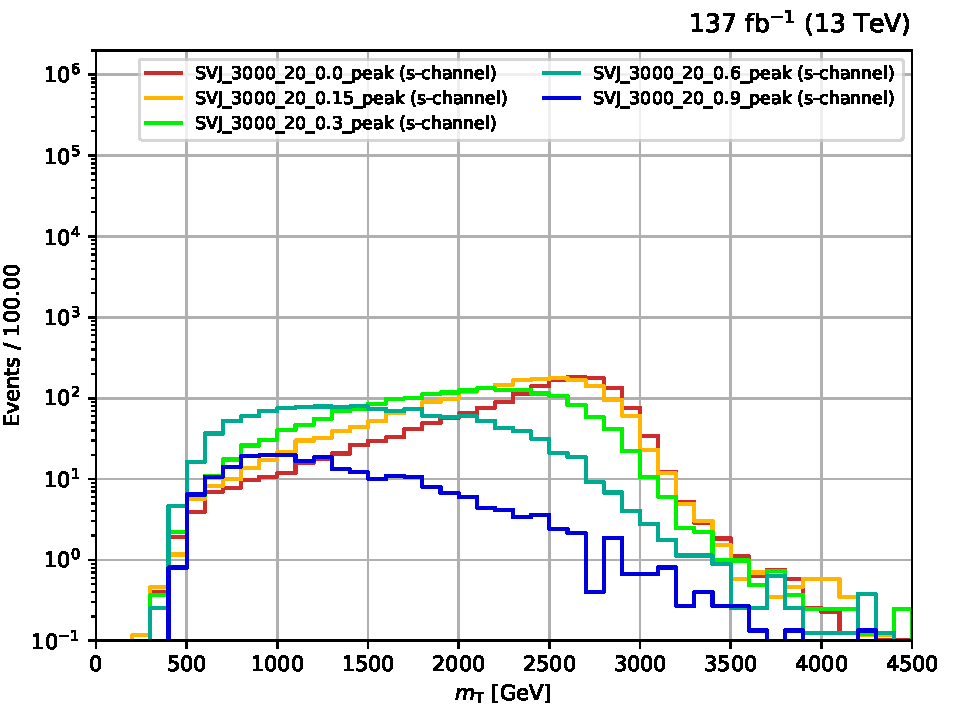
\includegraphics[width=\textwidth]{figures/s_channel_benchmark_variations/rinv.pdf}
        \caption{Varying \rinv}
    \end{subfigure}
    \hfill
    \begin{subfigure}[b]{0.48\textwidth}
        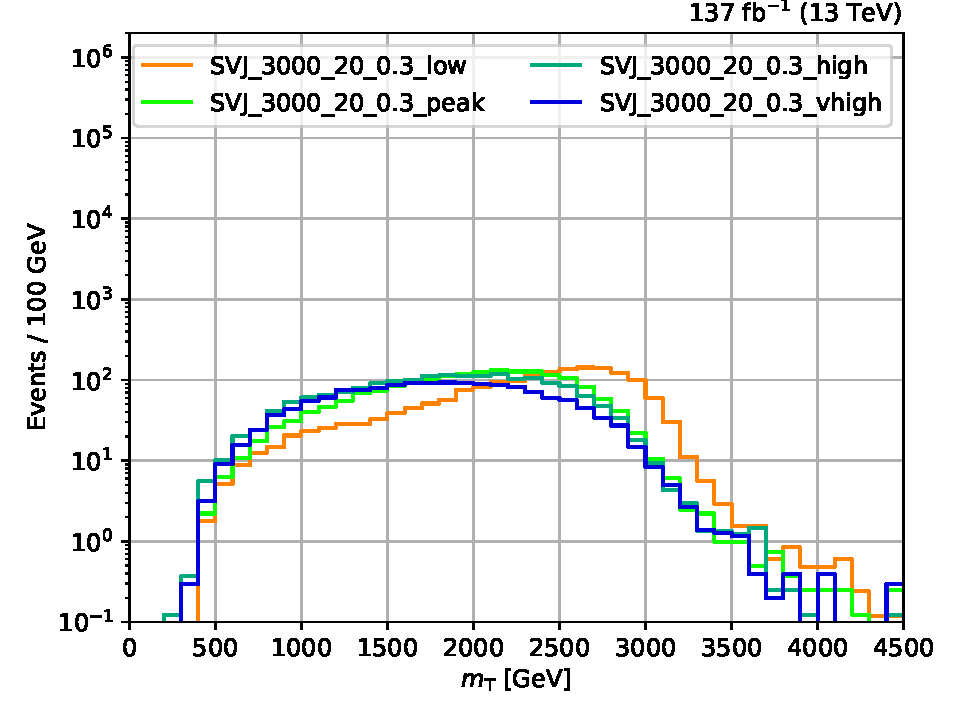
\includegraphics[width=\textwidth]{figures/s_channel_benchmark_variations/aD.pdf}
        \caption{Varying \aDark}
    \end{subfigure}
    \caption[Distributions of the transverse mass of the dijet system \mT for \schannel signal samples emulating the 2016 data taking period. In each panel, one of the free parameters of the semi-visible jets model is varied with respect to the benchmark point SVJ\_\-3000\_\-20\_\-0.3\_\-peak]{Distributions of the transverse mass of the dijet system \mT for \schannel signal samples emulating the 2016 data taking period. In each panel, one of the free parameters of the \glspl{svj} model is varied with respect to the benchmark point SVJ\_\-3000\_\-20\_\-0.3\_\-peak (red line).}
    \label{fig:svj_mg_benchmark_variations}
\end{figure}

% To help fill out parameter space, maybe add the following models (remember second variable is dark HADRON mass, not dark QUARK mass):
%   - Z' mass: 1000_20_0p3_peak (already have sample), 5000_20_0p3_peak
%   - dark hadron mass: 3000_4_0p3_peak, 3000_100_0p3_peak
%   - r_inv: 3000_20_0p0_peak, 3000_20_0p9_peak (already have sample)
%   - alpha dark: 3000_20_0p3_vlow (set to 0.25 * peak), 3000_20_0p3_vhigh (set to 2 * peak)
% Then I'd have 5 points per parameter. For colours, set dataset order such that it goes [lowest, low, benchmark, high, highest] for a given parameter. So benchmark is always the middle one and will be the same colour (green), and at least visually, the more red you go, the lower the parameter, and the more blue, the higher the parameter

% Dijet MT might not be the best to showcase the differences for some parameters, since MT essentially includes the met (and therefore the dark shower, which is clearly dependent on the Z' mass), and may not be sensitive to other changes. Could be good in the analysis, so we don't have to think too carefully about dark quark/hadron mass or alpha_d. Though, even though dark quark mass varied by factors of 2, still small compared to Z' mass which seems to be the most influential parameter. Other plots might be more telling, like showing how min_dphi changes with r_inv

% Lower r_inv is better at capturing Z' mass peak in MT


%=========================================================


\subsubsection{\texorpdfstring{\tchannel}{t-channel}}
\label{subsubsec:svj_signal_madgraph_tchannel}

% Here, I would describe the main properties of the t-channel model (the bifundamentals, dark quarks, couplings, etc.)

% Will have to decide whether to show s-channel and t-channel on same axes, or separately


%=========================================================


\subsection{Generation in \texorpdfstring{\PYTHIA}{Pythia}}
\label{subsec:svj_signal_pythia}

The \texttt{Hidden Valley} module allows for simulating $\HepProcess{\Pquark\APquark \to \PZprime \to \Pqdark\Paqdark}$, where the $\PZprime$ is acts as intended---a vector portal between the visible and dark sectors. Since we expect a small percentage of them to decay visibly, a branching ratio to each of the six \acrshort{sm} quarks is set to 0.003. The remaining fraction of 0.982 decays to $\Pqdark\Paqdark$, where $\Pqdark$ is a Hidden Valley particle charged only under that gauge group. The masses of the \PZprime and \Pqdark, and the narrow width of the \PZprime for resonance can be given. Showering in the dark and visible sectors is then performed as in Chpt.~\ref{subsec:svj_showering_pythia}. For both the complete event generation, and for hadronisation in the case of \MADGRAPH generation, \PYTHIA~8.230 was used.


%=========================================================


\subsection{Showering in \texorpdfstring{\PYTHIA}{Pythia}}
\label{subsec:svj_showering_pythia}

Once the hard process has been simulated, showering of the dark and visible particles is performed. This can be separated into three separate steps. The \emph{parton shower} itself is where undecayed quarks and gluons fragment due to colour confinement. At \emph{hadronisation}, the showered partons coalesce into composite hadrons. Finally, the \emph{underlying event} is the simulation of the previous two steps for additional, softer collisions from the hard scatter between initial state particles. Often, one just calls the sum of all of these steps the \emph{parton shower} or \emph{hadronisation}.

Dark quarks hadronise into one of two types of dark meson that correspond to particles from the \texttt{Hidden Valley} module: \Ppidark and \Prhodark, that are pseudoscalar and vector, respectively. Each possess flavour-diagonal and off-diagonal variants. They are generated with a ratio of 1:3 as the theory specifies the number of dark flavours $\Nf = \text{2}$. Dark hadrons are set to decay invisibly with a branching fraction \rinv. Remaining decay modes are to \acrshort{sm} quarks via a virtual \PZprime since it is the leptophobic portal between the dark and visible sectors. Decays of \Prhodark are democratic, i.e., with equal probability to accessible \acrshort{sm} quark-antiquark pairs.\footnote{Top quarks are excluded in all cases, since in the scan of model parameters where we predict the greatest sensitivity, the dark mesons are always too light to decay on shell to a \ttbar pair.} Specifically, \Prhodark particles with $\mDark > \text{2}m_{\Pbottom}$ have a $\text{1}/\text{5}$ probability to decay to a \Pup, \Pdown, \Pcharm, \Pstrange, or \Pbottom. For $2m_{\Pcharm} < \mDark < 2m_{\Pbottom}$, \Pbottom quarks are excluded and the branching ratio increases to $\text{1}/\text{4}$ for the remaining species. The \Pcharm quark is removed, and branching ratio modified, in the same manner for $\mDark < 2m_{\Pcharm}$.

The decays of the \Ppidark mesons, however, are through a mass insertion. They couple to the longitudinal component of the \PZprime, assumed to arise from a leptophobic Higgs sector in an analogous manner to the electroweak bosons. Running quark masses are accounted for---as calculated in Ref.~\citenum{QCD_ESW}--since the decays are produced at the Higgs mass scale. Branching fractions to the \acrshort{sm} quarks are therefore based on the squares of the \emph{running} masses over the \emph{pole} masses. A graphical representation of the mass insertion decay is provided in Fig.~\ref{fig:svj_mass_insertion}.

% The mass insertion is briefly mentioned in the theory paper. Vector dark hadrons can decay promptly to SM quarks through the vector portal via the Z'. But scalar and pseudoscalar decays are suppressed by the mass insertion. Not sure how this affects the t-channel

\begin{figure}[htbp]
    \centering
    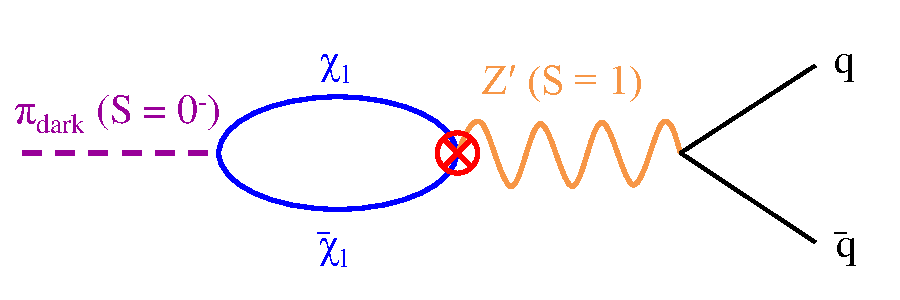
\includegraphics[width=0.5\textwidth]{figures/mass_insertion_diagram.pdf}
    \caption[A diagram of the mass insertion decay of \Ppidark mesons in the \schannel semi-visible jet model]{A diagram of the mass insertion decay of \Ppidark mesons in the \schannel \gls{svj} model.}
    \label{fig:svj_mass_insertion}
\end{figure}

We encode the dark confinement scale \lamDark and running dark coupling \aDark, based on the dark quark mass. \PYTHIA is now aware of the energy scales by which to hadronise and decay the dark sector particles. Final state dark radiation is also allowed, with a minimum \pt of $\text{1.1}\lamDark$.

% Why do we choose 1.1*Lambda_d for pt_min FSR?

The softer, visible radiation is simulated, and the clustering of \acrshort{sm} hadrons into \glspl{jet} happens. The procedure for clustering is known as ``sequential recombination'', where particles are successively combined until certain criteria are met. In \PYTHIA, clustering stops above the merging scale known as the \texttt{qCut}, which we set to 125\GeV. For events generated in \MADGRAPH and interfaced with \PYTHIA for the parton shower, it is recommended that $\texttt{qCut} > 1.1 \texttt{xqcut}$. Referring to the transverse momentum, the symbol $\kt$ is traditionally used in naming algorithms such as the \gls{antikt}. For consistency within this thesis, however, $\pt$ will be used.

For given particles $i$ and $j$, distance between them $d_{ij}$, and to the beam $d_{iB}$, are calculated as in Ref.~\citenum{schramm2016searching}:
\begin{equation}
    \begin{aligned}
d_{ij} &= \min(p_{\mathrm{T}i}^{2k}, \ p_{\mathrm{T}j}^{2k}) \frac{\Delta R_{ij}}{R^2},\\
d_{iB} &= p_{\mathrm{T}i}^{2k}
    \end{aligned}
    \label{eq:distances_kt_pythia}
\end{equation}

where, in the rapidity $y$-$\phi$ plane, $R$ is the radius of the cone (defined as 1.0 to match the merging parameters used in \MADGRAPH), $\Delta R_{ij}$ is the separation between $i$ and $j$,\footnote{This is calculated with Eq.~\ref{eq:delta_r} where $\eta$ is replaced with $y$ from Eq.~\ref{eq:rapidity_def}.} and $k$ defines the algorithm choice: $k = -\text{1}$ in the \gls{antikt}, $k = \text{0}$ in the Cambridge-Aachen algorithm, and $k = \text{1}$ in the $\kt$ algorithm. Our choice is the latter for the same purpose as as the cone radius size.

If $d_{ij} < d_{iB}$, the particles $i$ and $j$ are combined, replacing the individual constituents in the list of inputs. Otherwise, particle $i$ is designated as a jet and removed from list of inputs. For all combinations of particles remaining in the input list, the distances are recalculated until all objects possess a \pt above the merging scale. Once the algorithm has finished, we are left with fully-clustered \glspl{jet}. Matching is performed between the clustered jets and original partons to avoid double counting. Events with insufficiently-matched jets are rejected. A minimum number of \glspl{jet} may also be specified---two for this signal, since we expect a dijet final state---and events with fewer than this are rejected. A larger $\rinv$ tends to reduce the merging and matching efficiencies since more energy is locked in the dark sector and fewer jets are clustered above the merging scale.

% Might be interesting to adjust the merging scale based on the invisible fraction to get a higher efficiency. But that would be an extension for another student

% Look in AN for more description regarding the dark hadrons, decays of dark mesons, etc. (https://gitlab.cern.ch/tdr/notes/AN-19-061/-/blob/master/sections/sigsamples.tex)

% Describe effective parametrisation of Lambda_dark we use (and why - maximise number of dark hadrons?): Lambda_dark^peak = 3.2 * m_dark^0.8. Then use Eq.~\ref{eq:lambda_dark} to convert to alpha_dark^peak. Then we designate alpha_dark^low = 0.5 * alpha_dark^peak, and alpha_dark^high = 1.5 * alpha_dark^peak. Check the AN to ask exactly why we do this. Also note, that while we use low, peak and high, and they seem reasonably intuitive, there is support in my repository to just specify a number for alpha_d

\begin{figure}[htbp]
    \centering
    \includegraphics[width=0.5\textwidth]{figures/lambda_dark_vs_mDark.pdf}
    \caption[The dependence of the dark force scale \lamDark as a function of the dark hadron mass \mDark for each value of \aDark used in the analysis]{The dependence of the dark force scale \lamDark as a function of the dark hadron mass \mDark for each value of \aDark used in the analysis.}
    \label{fig:svj_lamDark_vs_mDark}
\end{figure}


%=========================================================


\subsubsection{Filtering events}
\label{subsubsec:svj_pythia_filters}

Two filters are implemented that reject events with unrealistic decays: a $Z_2$ symmetry in the model requires invisibly decaying dark hadrons to produce the dark matter particles in pairs, and an invisibly decaying \PZprime must do so into a $\Pqdark\Paqdark$ pair. Coupled with the efficiency of the \gls{jet} matching and clustering algorithms---which only significantly affects events generated externally and decayed with \PYTHIA---there are multiple sources of inefficiency in the generation.


%=========================================================


\subsection{\texorpdfstring{\PYTHIA}{Pythia}-\texorpdfstring{\MADGRAPH}{MadGraph} comparisons for \texorpdfstring{\schannel}{s-channel} signal}
\label{subsec:svj_schannel_comparisons}

% Adding discretionary hyphen to split the long SVJ labels and avoid overfull hboxes

\PYTHIAEIGHT is described as a multipurpose generator, meaning it has the flexibility to simulate many kinds of processes from \acrshort{qcd} and electroweak \acrshort{sm}, \acrshort{susy}, technicolour, and leptoquarks. Its status as the de facto standard for the parton shower and hadronisation means interfacing between that step and the hard process is simple. The use of Sudakov form factors and resummation also yield realistic jet structure. However, it is difficult to simulate processes more complex than \acrshort{lo}, and support for generating new models must sometimes be specifically added.

\MGvATNLO, on the other hand, is an automatic matrix element generator. It calculates the scattering matrix element for each subprocess for a given final state,\footnote{With our \glspl{svj} model, around 50 subprocesses exist for the \schannel mode, while approximately 820 exist for \tchannel.} with Feynman rules to generate each diagram within a subprocess. Integration if performed over the phase space for each subprocess to give the cross section. Generator and phase space level cuts are easy to implement, so that only signal in the phase space regions of interest are simulated. Systematic uncertainties from the generation step are also simple to extract, in the cases they are important to an analysis. High order processes, such as \acrshort{nlo}, and \acrshort{nnlo} can be simulated. While extremely taxing computationally, it is a straightforward implementation on the user side.

To verify that both \PYTHIA and \MADGRAPH are suitable generators, 100,000 events were generated for a selection of parameter points with each program independently. Six models encompassing a sufficient range of \mZprime, \mDark, and \rinv were chosen: SVJ\_\-1000\_\-20\_\-0.3\_\-peak, SVJ\_\-3000\_\-20\_\-0.1\_peak, SVJ\_\-3000\_\-20\_\-0.5\_\-peak, SVJ\_\-3000\_\-20\_\-0.9\_\-peak, SVJ\_\-3000\_\-50\_\-0.3\_\-peak, and SVJ\_\-4000\_\-20\_\-0.3\_\-peak. For all the simulation steps after the initial generation (described in more detail in Chpt.~\ref{subsec:cms_mc}), identical implementations were used. This was to compare the differences due only to the generator. No analysis-level selections were applied either for the same purpose.

Below are some of the important and insightful distributions for the \schannel production mode: the transverse mass of the dijet system \mT, the number of jets (with the large cone size equivalent to AK8 jets in the \gls{antikt}), the ratio of \MET to \mT, and the minimum azimuthal angle between the \MET and two leading \glspl{jet} $\dijetMindphi$. The ratio between the \MADGRAPH-generated and \PYTHIA-generated sample for a given model is also shown. For readability, plots are split into two sets comprising three models each. Fig.~\ref{fig:svj_mg_pythia_comparison_set1} showcases SVJ\_\-1000\_\-20\_\-0.3\_\-peak, SVJ\_\-3000\_\-20\_\-0.1\_\-peak, and SVJ\_\-3000\_\-20\_\-0.9\_\-peak, while Fig.~\ref{fig:svj_mg_pythia_comparison_set2} shows SVJ\_\-3000\_\-20\_\-0.5\_\-peak, SVJ\_\-3000\_\-50\_\-0.3\_\-peak, and SVJ\_\-4000\_\-20\_\-0.3\_\-peak.

\begin{figure}[htbp]
    \centering
    \begin{subfigure}[b]{0.48\textwidth}
        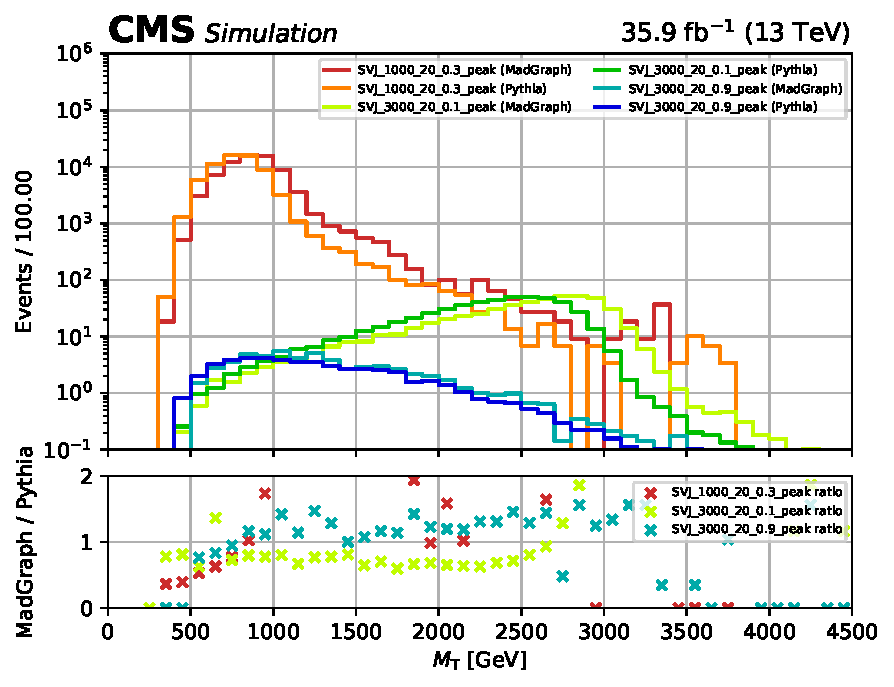
\includegraphics[width=\textwidth]{figures/madgraph_pythia_comparisons/with_ratios/part1/dijet_mt.pdf}
        \caption{Transverse mass of the dijet system}
    \end{subfigure}
    \hfill
    \begin{subfigure}[b]{0.48\textwidth}
        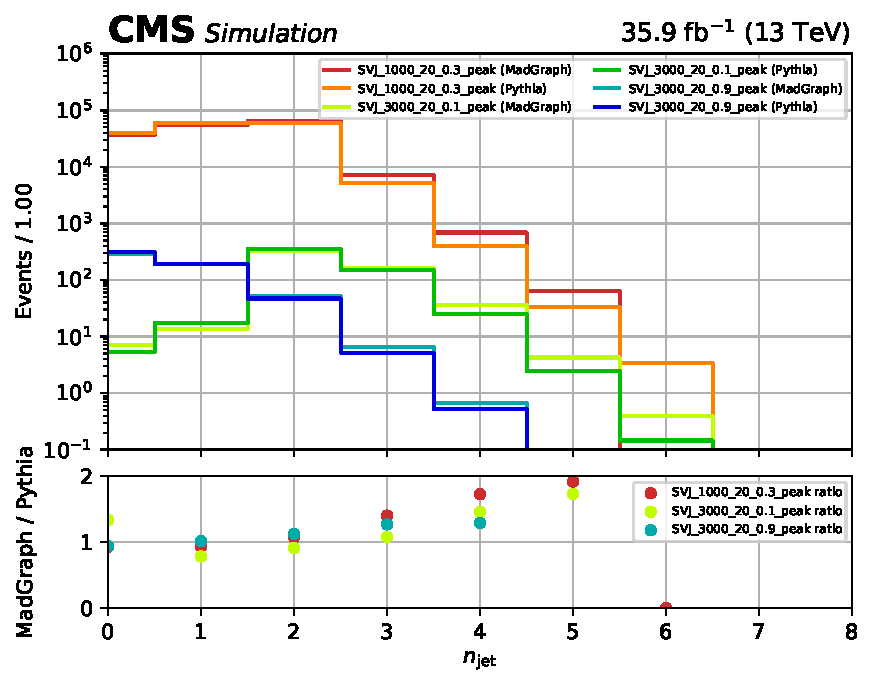
\includegraphics[width=\textwidth]{figures/madgraph_pythia_comparisons/with_ratios/part1/njet.pdf}
        \caption{\njet}
    \end{subfigure}

    \begin{subfigure}[b]{0.48\textwidth}
        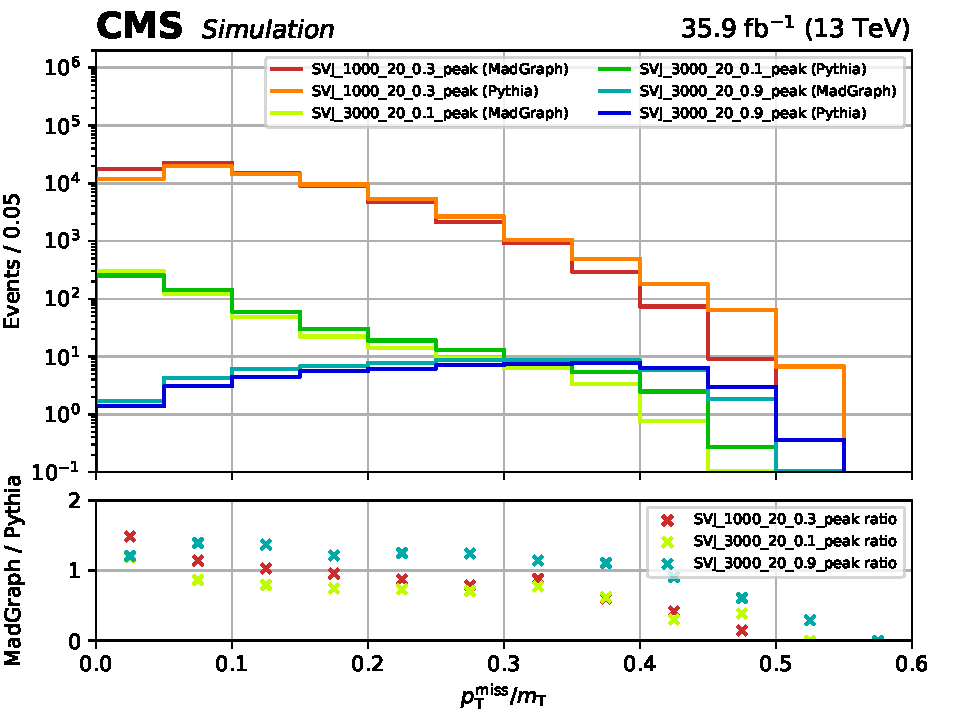
\includegraphics[width=\textwidth]{figures/madgraph_pythia_comparisons/with_ratios/part1/met_over_mt.pdf}
        \caption{$\MET/\mT$}
    \end{subfigure}
    \hfill
    \begin{subfigure}[b]{0.48\textwidth}
        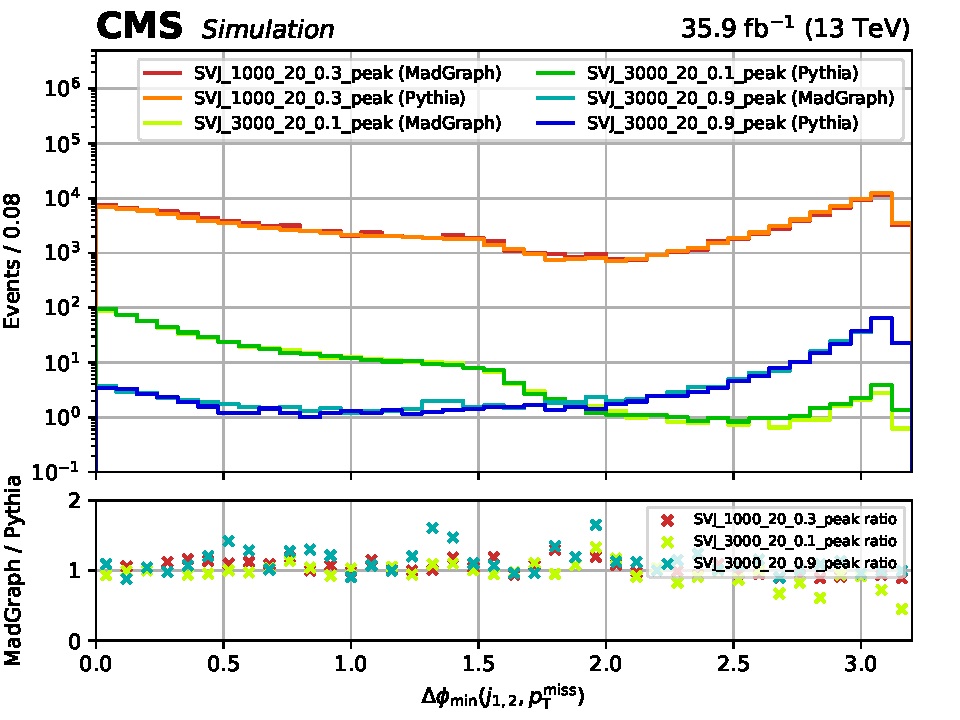
\includegraphics[width=\textwidth]{figures/madgraph_pythia_comparisons/with_ratios/part1/min_dphi.pdf}
        \caption{\mindphi between \MET and two leading \glspl{jet}}
    \end{subfigure}
    \caption[Distributions of several observables for the models SVJ\_\-1000\_\-20\_\-0.3\_\-peak, SVJ\_\-3000\_\-20\_\-0.1\_\-peak, and SVJ\_\-3000\_\-20\_\-0.9\_\-peak]{Distributions of several observables for the models SVJ\_\-1000\_\-20\_\-0.3\_\-peak, SVJ\_\-3000\_\-20\_\-0.1\_\-peak, and SVJ\_\-3000\_\-20\_\-0.9\_\-peak. Generation in \MGvATNLO is compared to \PYTHIAEIGHT, with the ratios between them for each model displayed in the respective subplot.}
    \label{fig:svj_mg_pythia_comparison_set1}
\end{figure}

\begin{figure}[htbp]
    \centering
    \begin{subfigure}[b]{0.48\textwidth}
        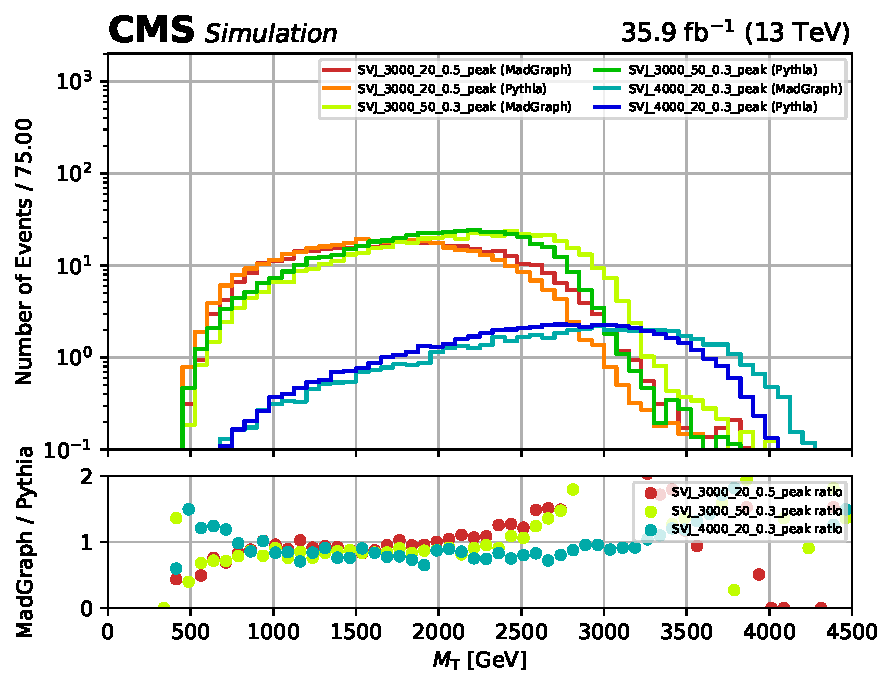
\includegraphics[width=\textwidth]{figures/madgraph_pythia_comparisons/with_ratios/part2/dijet_mt.pdf}
        \caption{Transverse mass of the dijet system}
    \end{subfigure}
    \hfill
    \begin{subfigure}[b]{0.48\textwidth}
        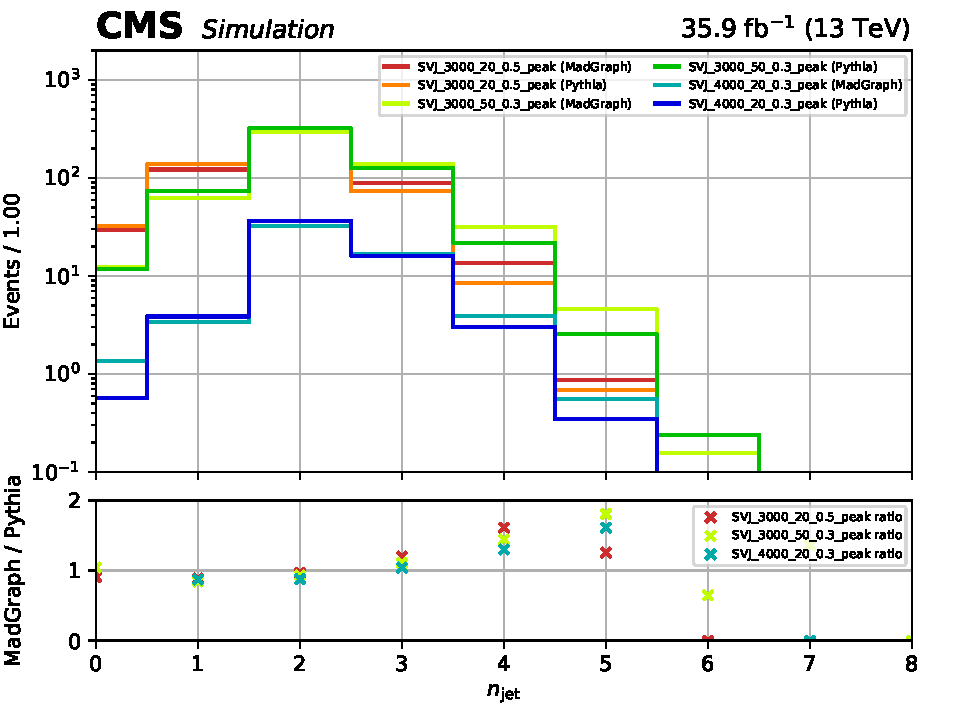
\includegraphics[width=\textwidth]{figures/madgraph_pythia_comparisons/with_ratios/part2/njet.pdf}
        \caption{\njet}
    \end{subfigure}

    \begin{subfigure}[b]{0.48\textwidth}
        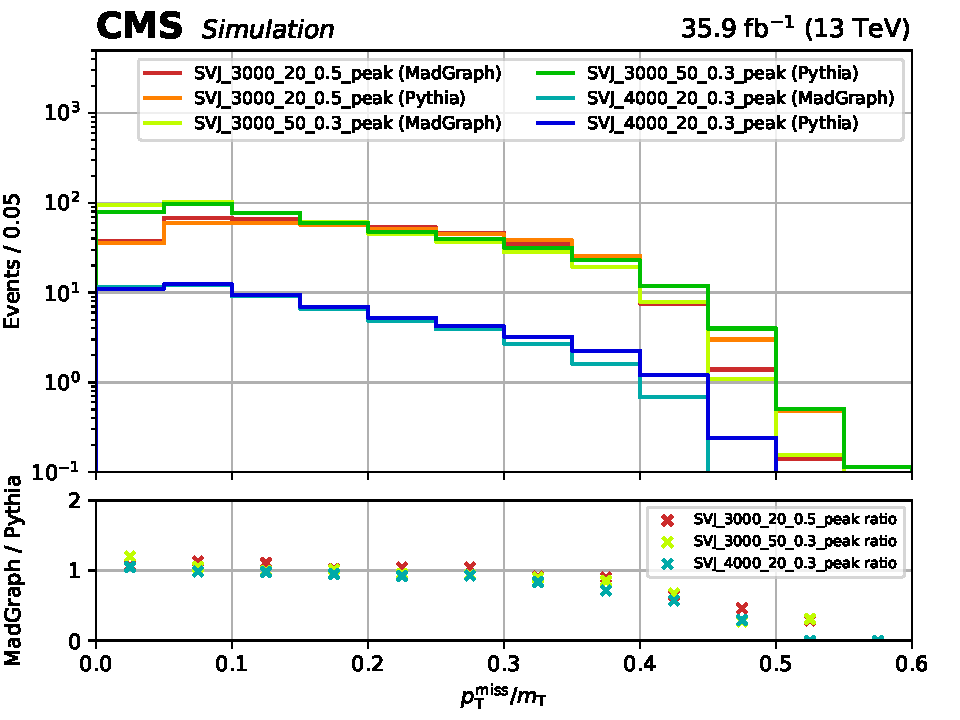
\includegraphics[width=\textwidth]{figures/madgraph_pythia_comparisons/with_ratios/part2/met_over_mt.pdf}
        \caption{$\MET/\mT$}
    \end{subfigure}
    \hfill
    \begin{subfigure}[b]{0.48\textwidth}
        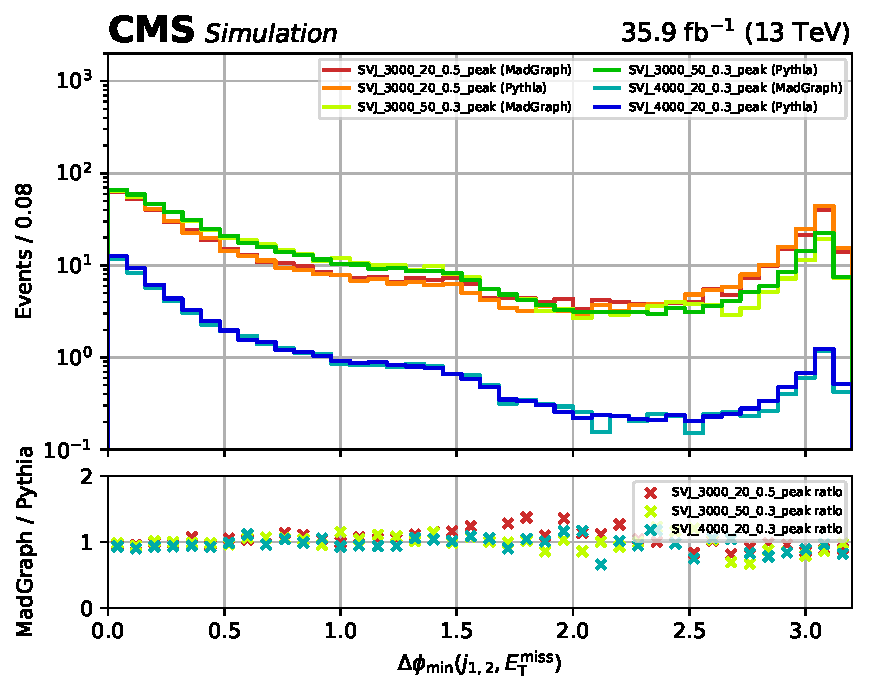
\includegraphics[width=\textwidth]{figures/madgraph_pythia_comparisons/with_ratios/part2/min_dphi.pdf}
        \caption{\mindphi between \MET and two leading \glspl{jet}}
    \end{subfigure}
    \caption[Distributions of several observables for the models SVJ\_\-3000\_\-20\_\-0.5\_\-peak, SVJ\_\-3000\_\-50\_\-0.3\_\-peak, and SVJ\_\-4000\_\-20\_\-0.3\_\-peak]{Distributions of several observables for the models SVJ\_\-3000\_\-20\_\-0.5\_\-peak, SVJ\_\-3000\_\-50\_\-0.3\_\-peak, and SVJ\_\-4000\_\-20\_\-0.3\_\-peak. Generation in \MGvATNLO is compared to \PYTHIAEIGHT, with the ratios between them for each model displayed in the respective subplot.}
    \label{fig:svj_mg_pythia_comparison_set2}
\end{figure}

% Most observables modelled quite well (also looked at MET, MHT, jet pt). Position variables such as eta and phi are basically identical, as expected.

% Differences in MT. Same kinda shape but looks shifted to higher energies in MadGraph. Might be a scale thing (need to tune xqcut/qcut?). Or may be something about the shower treating particles from MadGraph differently than those generated in Pythia

% Show that the min_dphi shows stuff similar to WIMPs for high r_inv (maximum at pi). And at low r_inv, peaks close to 0 and pi, so MET is likely to be within a jet or recoiling from it

% For njet, typically see 2 jets as expected. Sometimes, the shower of one dark quark can spread large enough to be clustered as two jets. Then there's ISR and FSR. 2D plots of dphi(j1/2/3, MET) vs njet or something might be interesting to see where the MET is aligned 

% Generating 100,000 events. Obviously fewer end up in the plots from jet matching and filter efficiency
